\section{Recommendation systems}
\only<presentation>{
  \begin{frame}
    \tableofcontents[ 
    currentsection, 
    hideothersubsections, 
    sectionstyle=show/shaded
    ] 
  \end{frame}
}

\begin{frame}
  \begin{figure}[H]
    \centering
    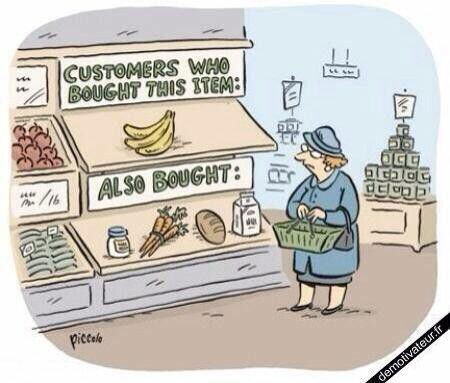
\includegraphics[width=0.4\textwidth]{../figures/recommendation}
    \only<article>{\caption{The recommendation problem}}
    \label{fig:recommendation}
  \end{figure}
  \only<article>{In many machine learning applications, we are dealing with the problem of proposing one or more alternatives to a human. The human can accept zero or more of these choices. As an example, when using an internet search engine, we typically see two things: (a) A list of webpages matching our search terms (b) A smaller list of advertisements that might be relevant to our search. At a high level, }
  \begin{block}{The recommendation problem}
    At time $t$
    \begin{enumerate}
    \item A customer $\bx_t$ appears. \only<article>{For the internet search problem, $\bx_t$ would at least involve the search term used.}
    \item We present a choice $a_t$. \only<article>{For the matching website, the choice is ranked list of websites. For the advertisements, however, it is typical }
    \item The customer chooses $y_t$. \only<article>{This might include selecting one or more of items suggested in $a_t$. The choice of the customer may not be directly visible.}
    \item We obtain a reward $r_t = \rho(a_t, y_t) \in \Reals$. \only<article>{Typically this is a payment either from the customer or an advertiser.}
    \end{enumerate}
  \end{block}
\end{frame}

\begin{frame}
  \begin{alertblock}{The two problems in recommendation systems}
    \begin{itemize}
    \item The modelling (or prediction) problem. \only<article>{Given the data, how to e.g. predict what movies a user likes and dislikes.}
    \item The recommendation problem. \only<article>{What movie(s) to actually recommend to a user.}
    \end{itemize}
    \only<article>{Although closely linked, those two problems have different evaluation metrics. The recommendation problem is harder, especially because the data do not tell us what our recommendation have been in the past, but only what users watched.}
  \end{alertblock}
\end{frame}


\begin{frame}
  \frametitle{How to predict user preferences?}
  \only<article>{In order for us to be able to provide good recommendations, we need to be able to predict user preferences. In the case of movies, preferences of a person for a movie can be expressed in terms of the hypothetical rating that a user would give to a movie. As Fig.~\ref{fig:user-ratings} shows, we frequently do have data about individual user ratings for movies, and we would like to somehow use those.}
  \begin{figure}[H]
    \centering 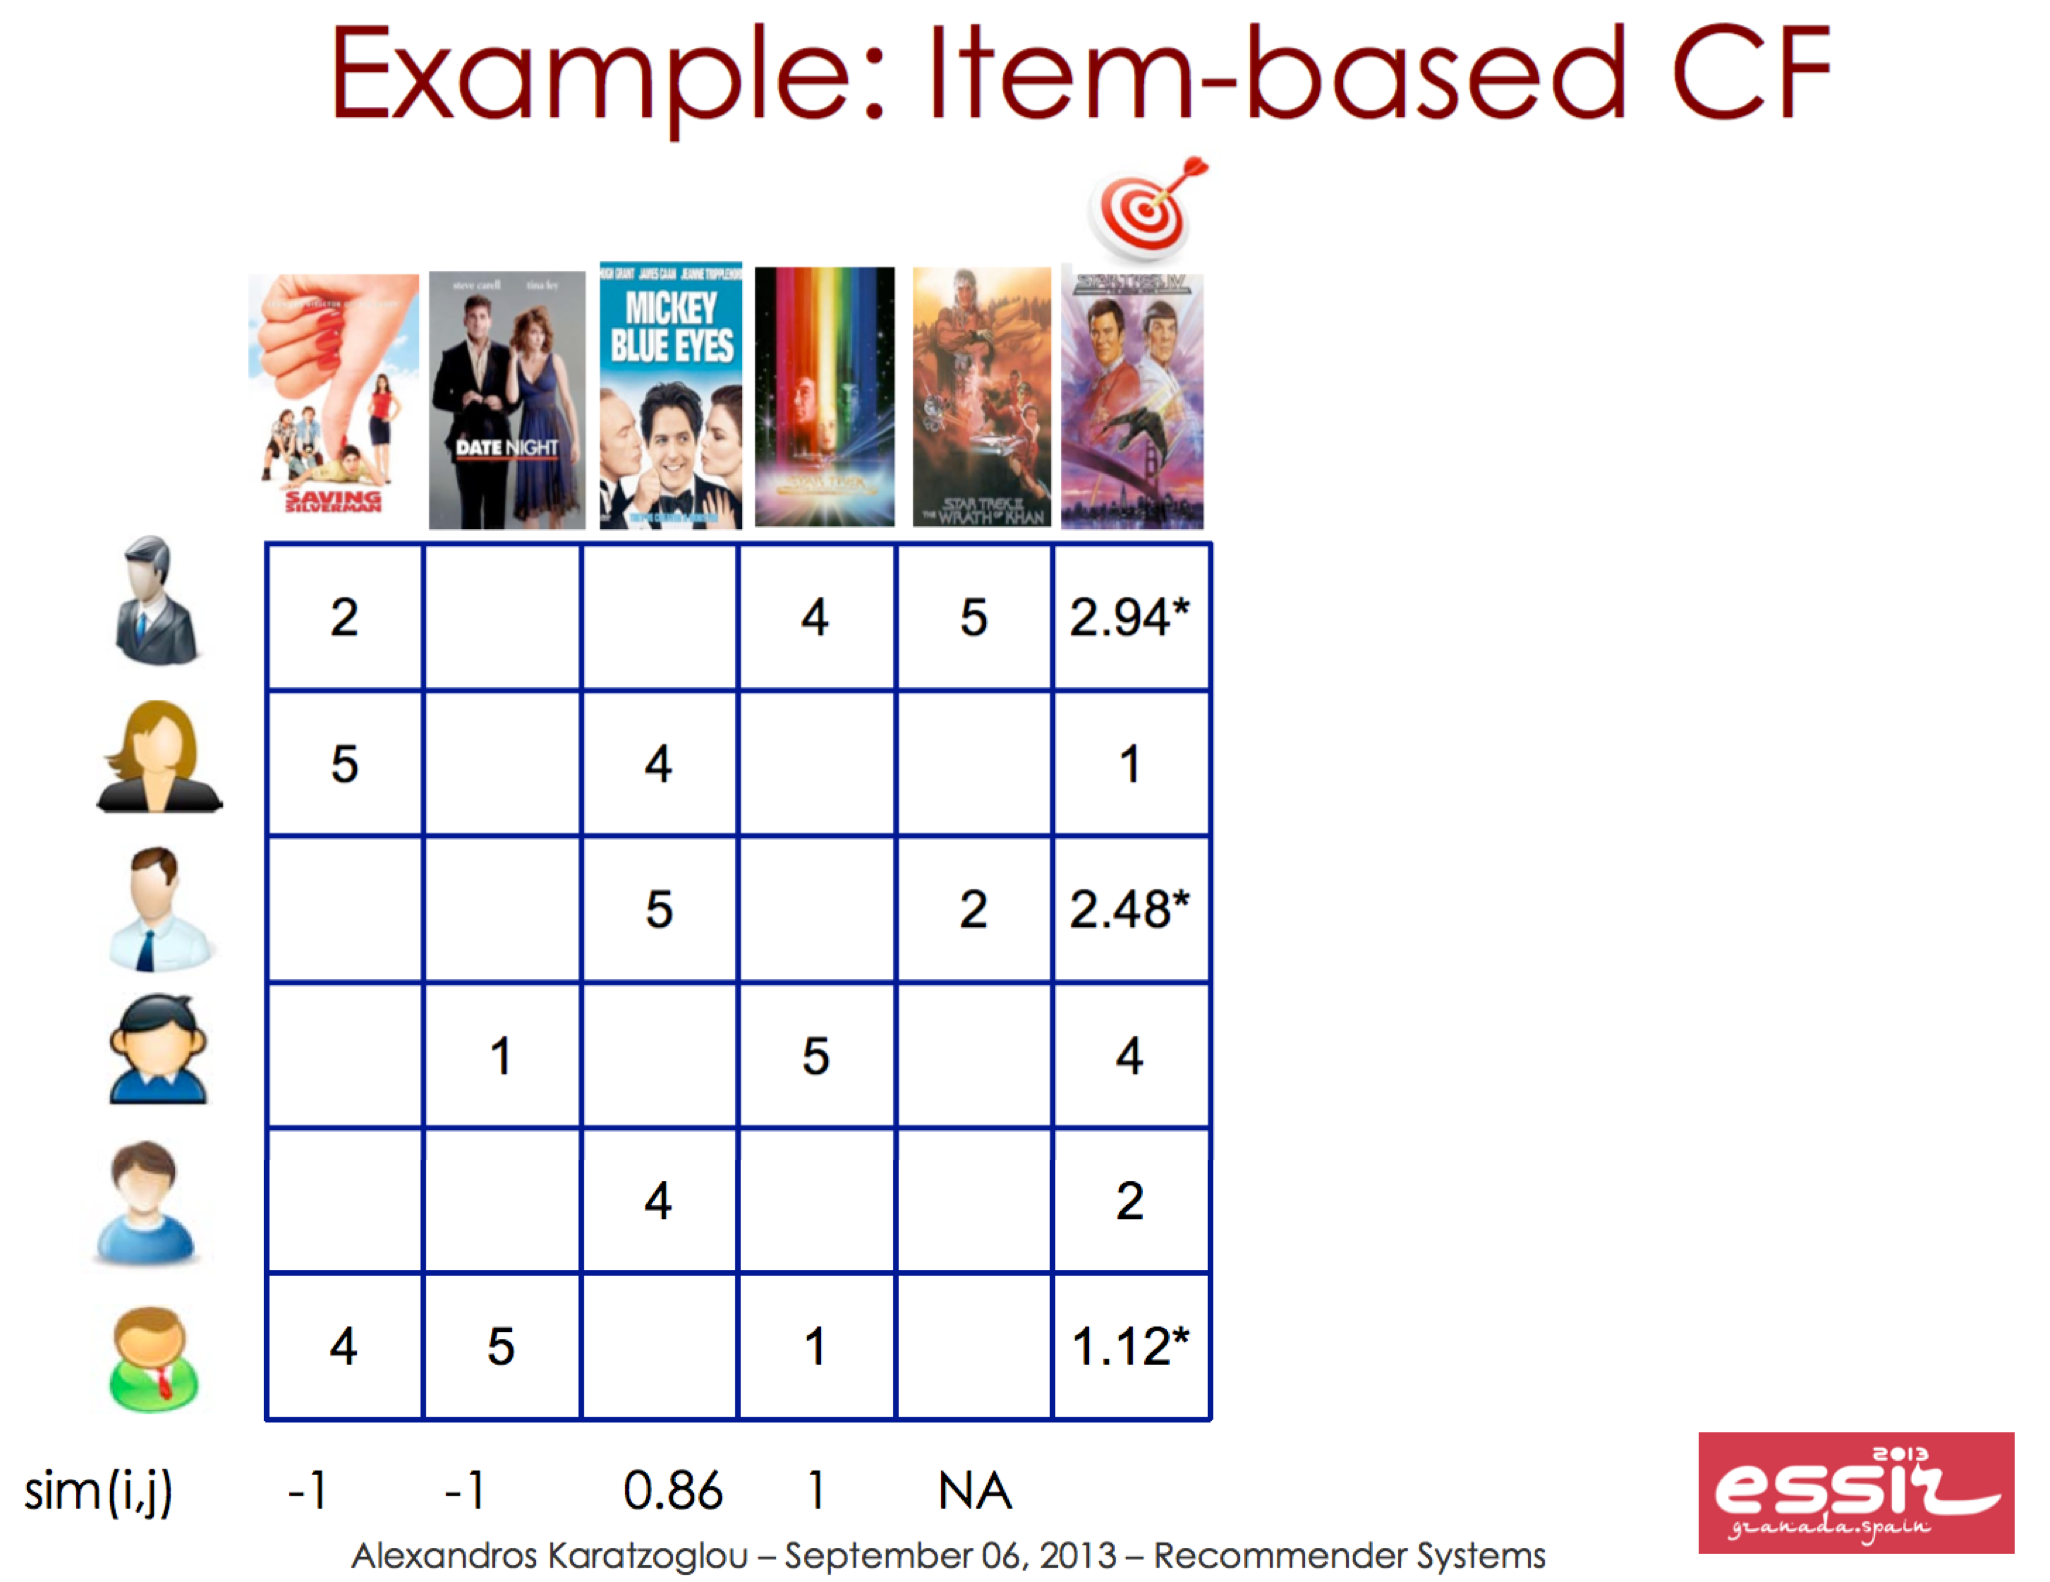
\includegraphics[width=0.9\textwidth]{../figures/recommendationExample-1}
    \caption{User ratings}
    \label{fig:user-ratings}
  \end{figure}

\end{frame}

\begin{frame}
  \begin{figure}[H]
    \centering
    
\includegraphics[width=0.9\textwidth]{../figures/netflix}
    \caption{What to recommend?}
    \label{fig:netflix}
  \end{figure}
  \only<article>{
    \begin{example}
      In the case of Netflix and related services, we would like to suggest movies to users which they are more likely to watch, as shown in Figure~\ref{fig:netflix}. However, how can we tell which movies those can be? It is probably not useful to just recommend them to rewatch a previously watched movie. We need to somehow take into account information across our user database: if somebody watched mostly the same films as you, then maybe you'd be interested in watching those movies she has that you haven't seen.

      In the Netflix catalogue, in particular, users also post reviews of the movies they have watched, as shown in Figure~\ref{fig:user-ratings}. This allows us to be able to guess the ratings of users from previous user's ratings.
    \end{example}
  }
\end{frame}



\begin{frame}
  \frametitle{Predictions based on similarity}
  \begin{block}{Content-based filtering.}
    \begin{itemize}
    \item Users typically like similar items. \only<article>{For example, a horror movie fan typically rates horror movies highly.}
    \item That means we can one user's ratings and \alert{item information} to predict their ratings for other items. \only<article>{In this scenario, we do not need to take into account the ratings of other people.}
    \end{itemize}
  \end{block}

  \begin{block}{Collaborative filtering}
    \begin{itemize}
    \item \alert{Similar users have similar tastes}. \only<article>{For example, consider two users $t, u$ who have each watched a set of movies $\CM_t$ and $\CM_u$ respectively, and $\CM_{t,u} = \CM_t \cap \CM_u$ is the set of common movies. If their ratings are the same for those movies, i.e. $x_{t.m} = x_{u,m} \forall m \in \CM_{t,u}$, then it's a good guess that they might have the same ratings for movies they have not both watched. }
    \item That means we can use similar user's \alert{ratings} to predict the ratings for other users. 
      \only<article>{The advantage is that ratings are readily available. The disadvantage is that new users have too few data to be matched to other users.}
    \end{itemize}
  \end{block}
\end{frame}


\begin{frame}
  \frametitle{$k$-NN for similarity}
  \begin{exercise}
    \begin{itemize}
    \item Define a distance $d : \CX^M \times \CX^M \to \Reals_+$ between user ratings.
    \item Apply a $k$-NN-like algorithm to prediction of user ratings from the dataset.
    \end{itemize}
  \end{exercise}
\end{frame}
\begin{frame}
  \begin{block}{Similarity between users}
    \only<article>{Let us define a similarity $w_{ij} \geq 0$ between two users so that}
    \[
    \sum_{j \neq i} w_{i,j} = 1,
    \qquad
    w^m_{i,j} \defn w_{i,j} \ind{x_{j,m}} / \sum_k w_{i,k} \ind{x_{k,m}}.
    \]
    \only<article>{There $w^m_{i,j}$ only considers those users who have rated movie $m$, so that $\sum_{j \neq i : x_{j,m} > 0} x^m_{i,j} = 1$. The overall similarity $w_i,j$ itself does not have to sum up to one, but it does need to be non-negative.}
  \end{block}

  \begin{example}[$k$-nearest neighbours]
    $w_{i,j} = 1/k$ for the $k$ nearest neighbours with respect to $d$.
  \end{example}


  \begin{example}[Weighted distance]
    \[
    w_{i,j} = \frac{\exp[-d(i,j)]}{\sum_{k \neq i} \exp[-d(i,j)]}
    \]
  \end{example}

  \begin{block}{Inferred ratings}
    \only<article>{Then we can define the inferred ratings to be the weighted average rating.}
    \[
    \hat{x}_{u.m} = \sum_{j \neq u} w^m_{u,j} x_{u,m}.
    \]
    \only<article>{But if the value $x_{u,m}$ is missing, we need to only}
  \end{block}
  
\end{frame}

\begin{frame}
  \begin{block}{A naive distance metric}
    \only<article>{A simple idea is to just look at the difference between the raw ratings in terms of the L1 norm:}
    \[
    d(i,j) \defn \|\bx_i - \bx_j\|_1.
    \]
    \only<article>{However this has the problem that this makes users who have watched different amounts of movies look very different.}
  \end{block}
  \begin{block}{Ignoring movies which are not shared.}
    \only<article>{
      We perhaps would only like to look at similarity for users with respect to which movies they have rated. This would lead to a distance such as}
    \[
    d(i,j) \defn \sum_{m} \ind{x_{i,m} \wedge x_{j,m}} |x_{i,m} - x_{j,m}|
    \]
  \end{block}
  \begin{block}{Using side-information}
    \only<article>{In some cases, we have additional information about the products or users. For example, users might be connected in a social network. Then we can tag users as similar if they are strongly connected, even if one of them has few or no movie ratings.}
    \only<presentation>{Social network data}
  \end{block}
  \begin{block}{Inferring a latent representation}
    \only<article>{Rather than going through specific algorithms for calculating similarities, we can think about learning a latent representation from the data. For example we could infer a network of users, and so a distance, from the individual ratings:}
    \[
    d(i,j) \defn f(\bx_i, \bx_j, \theta)
    \]
    \only<article>{More generally, we can try and infer some other latent representation.}
  \end{block}
\end{frame}

\subsection{Least squares representation}
\begin{frame}
  \frametitle{Latent representation}
  \begin{block}{The predictive model}
    \begin{itemize}
    \item $x_{um}$ rating of user $u$ for movie $m$.
    \item $r_{um} = \ind{x_{um} > 0}$ indicates which movies are rated.
    \item $\bz_{m} \in \Reals^n$: an $n$-dimensional representation of a movie.
    \item $\bc_{u} \in \Reals^n$: an $n$-dimensional representation of a user.
    \end{itemize}

    Given $\MC, \MZ$, our predicted movie rating can be written as
    \[
    \hat{x}_{u,m} \defn \bc_u^\top \bz_m, \qquad \hat{\MX} \defn \MC^\top \MZ.
    \]
    \only<article>{On the left side we have individual ratings and on the right side, in matrix form.}
  \end{block}
  \only<article>{We can now try and see how well this prediction fits the data for a movie. One idea is to simply use $|\hat{x}_{m,u} - x_{m,u}|$ to show the difference between the prediction and the actual rating. 
    Now can now define the prediction \alert{error} for a given representation $\MC, \MZ$ as}
  \[
  f(\MC, \MZ) = \|(\MR \circ \hat{\MX} - \MR \circ \MX)^\top (\MR \circ \hat{\MX} - \MR \circ\MX)\|_1
  \]

  \only<article>{Here multiplying with the $\MR$ matrix ensures that we ignore pairs with no ratings.
    \begin{block}{Alternating Least Squares~\cite{takacs2012alternating}}
      \begin{align}
        \label{eq:als}
        \MC_{t+1} &= \argmin_{\MC} f(\MC, \MZ_t) + \lambda g(\MZ, \MZ_t)\\
        \MC_{t} &= \argmin_{\MZ} f(\MC_t, \MZ) +  + \lambda g(\MZ_t, \MZ)
      \end{align}
    \end{block}
  }
\end{frame}


\subsection{Preferences as a latent variable}
\begin{frame}
  \frametitle{A simple preference model}
  \only<article>{As a simple model, we can assume that each person belongs to a \alert{type}. Every type has the same preferences over films. In the simplest possible model, a user of type $c_i$ that has watched a movie $m$ will rate the film deterministically $x_{c,m}$. More generally, we can assume the following model.}
  \begin{figure}[H]
    \centering
    \begin{tikzpicture}
      \node[RV] at (2,0) (data) {$\bx_t$};
      \node[RV,hidden] at (0,0) (cluster) {$c_{t}$};
      \draw[->] (cluster)--(data);
      \uncover<2>{
        \node[RV,hidden] at (2,1) (param) {$\param$};
        \draw[->] (param)--(cluster);
        \draw[->] (param)--(data);
      }
    \end{tikzpicture}
    \caption{Basic preference model}
    \label{fig:basic-preference-model}
  \end{figure}
  \begin{example}[Discrete preference model]
    \begin{itemize}
    \item User type $c \in \CC$. \only<article>{For simplicity, we can think of there being a finite number of types $\CC = \{1, \ldots, n\}$.}
    \item User ratings  $\bx$ with $x_{m} \in \CX = \{0, 1\}$ rating for movie $m$.
    \item Preference distribution 
      \[
      P_\param(\bx | \bc) = \prod_{m=1}^M \param_{m,c}^{x_m} (1 - \param_{m,c})^{(1 - x_m)}.
      \]
    \item $P_\param(c) = \param_c$, $\sum_c \param_c = 1$.
    \end{itemize}
  \end{example}
\end{frame}

\begin{frame}
  \frametitle{A more complex preference model}
  \only<article>{As a simple model, we can assume that each person belongs to a \alert{type}. Every type has the same preferences over films. In the simplest possible model, a user of type $c_i$ that has watched a movie $m$ will rate the film deterministically $x_{c,m}$. More generally, we can assume the following model.}
  \begin{figure}[H]
    \centering
    \begin{tikzpicture}
      \node[RV] at (2,0) (data) {$x$};
      \node[RV,hidden] at (0,0) (cluster) {$c$};
      \node[RV,hidden] at (4,0) (movie) {$z$};
      \draw[->] (cluster)--(data);
      \draw[->] (movie)--(data);
      \node[RV,hidden] at (2,1) (param) {$\param$};
      \draw[->] (param)--(cluster);
      \draw[->] (param)--(data);
      \draw[->] (param)--(movie);
    \end{tikzpicture}
    \caption{Preference model}
    \label{fig:preference-model}
  \end{figure}
  \begin{block}{Preference model}
    \begin{itemize}
    \item User type $\bc \in \CC$. \only<article>{For simplicity, we can think of there being a finite number of types $\CC = \{1, \ldots, n\}$.}
    \item Movie type $\bz \in \CZ$.
    \item Preference distribution 
      \[
      P_\param(x | \bc, \bz) = \Normal(\bc^\top \bz, \sigma_\theta)
      \]
    \item Feature prior
      \[
      P_\param(\bc) = \Normal(0, \lambda_\theta)
      \]
    \end{itemize}
  \end{block}

  
\end{frame}


\subsection{The recommendation problem}

\begin{frame}
  \frametitle{What to recommend}
  \begin{figure}[H]
    \centering
    \begin{tikzpicture}
      \node[RV] at (2,0) (data) {$\bx$};
      \node[RV,hidden] at (2,-1) (movie1) {$x_1$};
      \node[RV,hidden] at (2,-2) (movie2) {$x_2$};
      \node[RV,hidden] at (0,0) (cluster) {$c$};
      \node[RV,hidden] at (4,0) (movie) {$z$};
      \draw[->] (cluster)--(data);
      \draw[->] (movie)--(data);
      \draw[->] (cluster)--(data);
      \draw[->] (movie)--(movie1);
      \draw[->] (movie)--(movie2);
      \draw[->] (cluster)--(movie1);
      \draw[->] (cluster)--(movie2);
    \end{tikzpicture}
    \caption{Preference model}
  \end{figure}
  \begin{block}{The recommendation problem for a given $\param$}
    \uncover<2->{
      \begin{align}
        \max_\pol \E^\pol_\param(U \mid \bx)
        &=
          \max_a \sum_{c, z} U(a, y) \alert{\Pr(y \mid a, c, z)} P_\param(c, z \mid \bx)\\
        &=
          \max_a \sum_{c, z} U(a, y) \sum_{x_a} \alert{\Pr(y \mid a, x_a)} P_\param(x_a \mid c, z) P_\param(c, z \mid \bx)
      \end{align}
    }


  \end{block}
\end{frame}


\begin{frame}
  \frametitle{Two ways to model the effect of actions}
  \begin{figure}[H]
    \centering
    \begin{tikzpicture}
      \node[RV] at (2,0) (data) {$\bx$};
      \node[RV,hidden] at (0,0) (cluster) {$c$};
      \node[RV,hidden] at (4,0) (movie) {$z$};
      \draw[->] (cluster)--(data);
      \draw[->] (movie)--(data);
      \draw[->] (cluster)--(data);
      \node[select] at (-2,0) (action) {$a$};
      \node[RV] at (0,-2) (outcome) {$y$};
      \draw[->] (action) -- (outcome);
      \only<1>{
        \node[RV,hidden] at (2,-1) (movie1) {$x_1$};
        \node[RV,hidden] at (2,-2) (movie2) {$x_2$};
        \draw[->] (movie)--(movie1);
        \draw[->] (movie)--(movie2);
        \draw[->] (cluster)--(movie1);
        \draw[->] (cluster)--(movie2);
        \draw[->] (movie1)--(outcome);
        \draw[->] (movie2)--(outcome);
      }
      \only<2>{
        \draw[->] (cluster)--(outcome);
        \draw[->] (movie)--(outcome);
      }
    \end{tikzpicture}
    \caption{Preference model}
  \end{figure}
  \only<presentation>{
    \begin{align}
      \E_\param (U \mid a, \bx) =
      \only<2>{
      \sum_{c, z} U(a, y) \alert{\Pr(y \mid a, c, z)} P_\param(c, z \mid \bx)
      }
      \only<1>{
      \sum_{c, z} U(a, y) \sum_{x_a} \alert{\Pr(y \mid a, x_a)} P_\param(x_a \mid c, z) P_\param(c, z \mid \bx)
      }
    \end{align}
  }
  \only<article>{
    What is the right model for the effects of our actions? In the most general case, the model could depend on the complete set of latent ratings of all the movies. However, it is hard to interpret this, as the user is also probably not aware of what these ratings are themselves. So it seems simpler and more appropriate to predict the outcome based on our action and the latent representation, especially since we will be marginalising over the individual ratings anyway.}
\end{frame}




  %%% Local Variables:
  %%% mode: latex
  %%% TeX-engine: xetex
  %%% TeX-master: "notes.tex"
  %%% End:
